\chapter{Personalized Expected Utility: COMING SOON}
\label{ch-personalized-test}


\url{https://ftp.cs.ucla.edu/pub/stat_ser/r507.pdf}

\beq
P_{y_0, y_1|z}=
P(\rvy_0=y_0, \rvy_1=y_1|z)
\eeq

$\alp_{y_0, y_1}$ utility function

conditional expected utility

\beq
EU_z = E_{\rvy_0,\rvy_1|z}[\alp_{\rvy_0,\rvy_1}]=\alp_{i,j}P_{i,j|z}
\eeq

\beq
Uplift = ATE_z = E_{1|1,z}-E_{1|0,z}
\eeq



\beq
\begin{array}{lll}
\beta = \alp_{0,1} &(y_0=0, y_1=1)& \text{ compliers }
\\
\gamma = \alp_{1,1}&(y_0=1, y_1=1) & \text{ always takers} 
\\
\theta = \alp_{0,0}& (y_0=0, y_1=0&\text{ never takers})
\\
\delta = \alp_{1,0}& (y_0=1, y_1=0)&\text{ defiers}
\end{array}
\eeq

\beq 
\xymatrix@C=4pc{
\rvy_0=0\ar@{-}@/^1pc/[dr]|{\alp_{0,1}}
\ar@{-}[r]^{\alp_{0,0}}
&\rvy_1=0
\\
\rvy_0=1\ar@{-}@/_1pc/[ur]|{\alp_{1,0}}
\ar@{-}[r]_{\alp_{1,1}}
&
\rvy_1=1
}
\eeq

\section{Goal of PEU Theory}
\begin{figure}[h!]
\centering
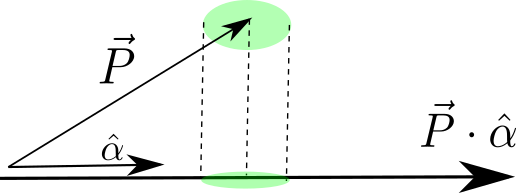
\includegraphics[width=2.5in]
{personalized-test/utility.png}
\caption{Bounds 
on the probability
vector $\vec{P}$
induce bounds on dot 
product $EU=\vec{P}\cdot \hat{\alpha}$.
Here $\hat{\alp}$ is a unit vector
that stands for a normalized 
utility function, and
$EU$ stands for the expected utility.
} 
\label{fig-utility}
\end{figure}

\section{Bnets for PEU Theory}




\section{Bounds for unspecified bnet}
balanced  utility
\beq
\alp_B = \alp_{0,0} + \alp_{1,1}
\eeq

unbalanced utility
\beq
\alp_U =
\alp_{1,0}+\alp_{0,1}
\eeq

\beq
\s = \alp_U - \alp_B
\eeq

\beq
\alp_{1-0, j}=\alp_{1,j} -\alp_{0,j}
\eeq

\beq
\alp_{j,1-0}=\alp_{j,1} -\alp_{j,0}
\eeq


\begin{claim}

{\renewcommand\arraystretch{1.5}
\beq
\left\{
\begin{array}{ll}
\max p_{[1\ldots4]}
\leq
EU_z
\leq
\min p_{[5\ldots 8]}
&\text{ if } \s<0
\\
\max p_{[5\ldots 8]}
\leq
EU_z
\leq
\min p_{[1\ldots 4]}
&\text{ if } \s>0
\end{array}
\right.
\eeq
}
where\footnote{$p_{[a\ldots b]}=(p_a, p_{a+1}, \ldots p_b)$
for integers $a, b$ such that $a<b$.}

{\renewcommand\arraystretch{1.5}
\beq
\left\{
\begin{array}{l}
p_1=\alp_{0, 1-0}E_{1|1,z} +
\alp_{j,0}E_{j|0,z}
\\
p_2=
\alp_{0-1,1}E_{0|0,z}
+ \alp_{1,j}E_{j|1,z} 
\\
p_3 =p_5
+\s O_{*,*|z}
\\
p_4 = p_1
-\s E_{1|0,z}
+ \s (1-O_{*,*|z})
\end{array}
\right.
\eeq
}

{\renewcommand\arraystretch{1.5}
\beq
\left\{
\begin{array}{l}
p_5 =

\alp_{1, 1-0}E_{1|1,z} 
+\alp_{j,0}E_{j|0,z}
\\
p_6 = 
p_1
-\s E_{1|0,z}
\\
p_7 =p_5
-\s E_{1|0,z}
+\s P(\rvy=1|z)
\\
p_8 = p_1
-\s P(\rvy=1|z)
\end{array}
\right.
\eeq
}

\end{claim}
\proof
\qed

monotonicity

\beq
P(\rvy_0=1, \rvy_1=0)=0
\eeq


\begin{claim}
In general,

\beq
P_{0,0|z}=E_{0|1,z}-P_{1,0|z}
\eeq

\beq
P_{1,1|z}=E_{1|0,z}-P_{1,0|z}
\eeq

\beqa
P_{0,1|z}
&=&
1-P_{0,0|z}-P_{1,1|z}-P_{1,0|z}
\\
&=&
 1-E_{0|1,z}-E_{1|0,z}+P_{1,0|z}
\eeqa


\end{claim}
\proof

\beq
P_{1,0|z}
 + \underbrace{P_{0,1|z} + P_{1,1|z}}_
{= P(\rvy_1=1|z)}+ P_{0,0|z}=1
\eeq
Hence 
\beqa
P_{0,0|z}&=&1-P(\rvy_1=1|z)-P_{1,0|z}
\\
&=&P(\rvy_1=0|z)-P_{1,0|z}
\\
&=&
E_{0|1,z}-P_{1,0|z}
\eeqa

\beq
P_{1,0|z}
 + \underbrace{P_{0,1|z} + P_{0,0|z}}_
{= P(\rvy_0=0|z)}+ P_{1,1|z}=1
\eeq
Hence 
\beqa
P_{1,1|z}&=&1-P(\rvy_0=0|z)-P_{1,0|z}
\\
&=&P(\rvy_0=1|z)-P_{1,0|z}
\\
&=&
E_{1|0,z}-P_{1,0|z}
\\
\eeqa

\qed

If monotonicity holds,
or $\alp_{1,0}=0$,

\beq
EU_z = \alp_{0,0}P_{0,0|z}
+\alp_{1,1}P_{1,1|z}
+\alp_{0,1}P_{0,1|z}
+
\underbrace{\alp_{1,0}P_{1,0|z}}_{=0}
\eeq


\begin{claim}

\beq
EU_z = \alp_{0,0} 
\underbrace{E_{0|1,z}}_{=1-E_{1|1,z}}
+ \alp_{1,1}E_{1|0,z}
+ \alp_{0,1}
\underbrace{( 1-E_{0|1,z}-E_{1|0,z})}
_{= E_{1|1,z}-E_{1|0,z}=ATE_z}
+ \s P_{1,0|z}
\eeq
Hence, if monotonicity holds,
or $\s=0$,
\beq
(EU_z)_{\s=0} = \alp_{0,0} E_{0|1,z}
+ \alp_{1,1}E_{1|0,z}
+ \alp_{0,1}ATE_z
\eeq
\end{claim}
\proof
In general,
\beq
EU_z =
\left\{
\begin{array}{r}
\quad\alp_{0,0}P_{0,0|z}
\\
+\alp_{1,1}P_{1,1|z}
\\
+\alp_{0,1}P_{0,1|z}
\\
+\alp_{1,0}P_{1,0|z}
\end{array}
\right.
=
\left\{
\begin{array}{l}
\quad\alp_{0,0}(E_{0|1,z}-P_{1,0|z})
\\
+\alp_{1,1}(E_{1|0,z}-P_{1,0|z})
\\
+\alp_{0,1}(1-E_{0|1,z}-E_{1|0,z}+P_{1,0|z})
\\
+\alp_{1,0}P_{1,0|z}
\end{array}
\right.
\eeq
Hence,
\beq
EU_z = (EU_z)_{\s=0} + \s P_{1,0|z}
\eeq

\qed

\section{Bounds for specific bnet  families}


